\documentclass{article}
\usepackage[T1]{fontenc}
\usepackage{lmodern}
\usepackage{graphicx}
\usepackage{amsmath,amssymb}
\usepackage[a4paper,margin=2cm]{geometry}
\usepackage[absolute,overlay]{textpos}
\setlength{\TPHorizModule}{1mm}
\setlength{\TPVertModule}{1mm}
\usepackage[indonesian]{babel}
\usepackage{hyperref}
\setlength{\emergencystretch}{2em}
% unit: Halaman 1

\begin{document}

% === Halaman 1 (llm) ===

\begin{center}
Bahan kuliah IF4020 Kriptografi

\Huge \textcolor{red}{03 -- Kriptografi Klasik}
\Large \textcolor{red}{(Bagian 1)}

\vspace{10mm}

\large Oleh: Rinaldi M

\vspace{20mm}

\textbf{Program Studi Teknik Informatika}\\
\textbf{Sekolah Teknik Elektro dan Informatika}\\
\textbf{Institut Teknologi Bandung}\\
\textbf{2026}
\end{center}

% deskripsi: Ilustrasi kunci kriptografi klasik berupa silinder logam dengan cincin huruf yang dapat diputar (cipher disk/cylinder).
% bbox normalisasi: [0.0470, 0.4520, 0.2860, 0.7090]
\begin{textblock*}{50.19mm}(9.87mm,134.24mm)
\noindent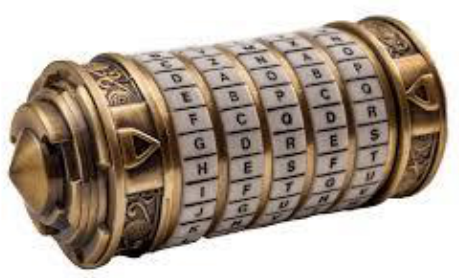
\includegraphics[width=50.19mm,height=76.33mm]{../../images/llm/page_001_img_01.png}%
\end{textblock*}

\end{document}
